\subsection{Clustering of a long trajectory (proof of concept)}
\label{sec:pyproct_supp_5}

In a cluster analysis, the function distance must be applied many
times to the different elements of the dataset. As pyProCT needs to
generate numerous clusterings, it is unfeasible to use an `on line'
distance calculation approach. Instead, the symmetric pairwise distance
matrix is calculated once and used throughout all the process, improving
the overall performance. The size of the distance matrix grows quadratically
in the size of the input (the number of conformations), and can rapidly
consume all the RAM of a state-of-the-art workstation. Because of
this, using pyProCT with large conformational ensembles supposes a
technical challenge.

In Section 3.2 we have shown how this limitation can be overcome by
performing a redundancy reduction on the input trajectory before analyzing
the dataset. Here we want to apply this technique to reduce a longer
trajectory (more than 1million frames) to an easier to handle size.


\subsubsection{The trajectory}

We used the 206 $\mu$s trajectory of Trp-cage (PDB%
\footnote{Protein Data Bank (http://www.rcsb.org)%
} id 2JOF) presented in an article from D. E. Shaw's group \cite{kresten_lindorff-larsen1_how_2011}.
The details of the simulation can be found in the Supporting Online
Materials for this article.


\subsubsection{Redundancy elimination}

\begin{figure}
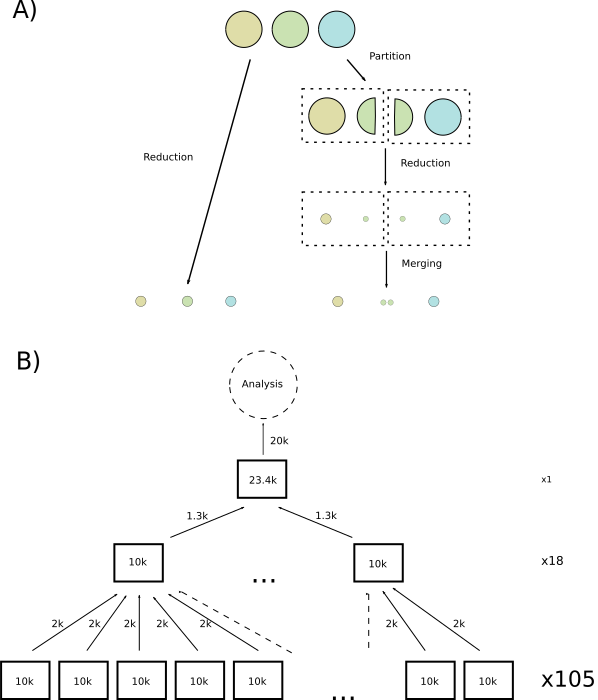
\includegraphics[width=\textwidth,height=\textheight,keepaspectratio]{pyproct_supp_compression.pdf}

\caption{A) Global reduction of the size of the dataset vs. merging local reductions. B) Different levels of compression including the number of frames used in each level.}
\label{fig:compression}
\end{figure}

The goal of this technique is to reduce the input trajectory by exchanging
sets of similar conformations (clusters) by a choice of its most representative
structures so that the final number of elements is proportional to
the original size of the cluster.

The first step to apply the reduction is to produce a clustering.
This makes us face the memory problem mentioned before. A workaround
for this issue is to divide the trajectory into smaller parts so that
each distance matrix can fit in memory, process each part separately
and then merge them again. Unfortunately, arbitrarily partitioning
the trajectory can separate elements that could form part of the same
cluster (which is more prone to happen in the boundaries of each part).
This can lead to an unevenness in the redundancy elimination process
(see the 2D example in Fig. \ref{fig:compression}A). We have performed
the reduction process iteratively to mitigate the problem. We start
with 105 parts of almost 10k frames each. After reducing each part
to 2k frames, we merged them into groups of 7 (\around14k
frames each). These groups were compressed to have around 1.3k frames
each and merged again to form a \around24k frames trajectory.
This was finally reduced to 20k frames and then analyzed. 


\subsubsection{Results}


\subsubsubsection{Performance}

pyProCT was run in an Intel Xeon CPU W3530 @ 2.80GHz workstation.
Each run of pyProCT spawned a maximum of 6 processes. While it was
being executed the workstation was normally used, occasionally triggering
operating system's swap mechanisms, which slowed down the process.
Therefore, the calculated execution time has merely a qualitative
meaning (see Table \ref{tab:results}). Also, the lack of knowledge of the
system forced us to use a very general hypothesis, increasing the
number of clusterings that had to be generated and thus the total
execution time. 

\begin{table}
\centering
\begin{tabular}{ r c c c }
\toprule
Level & Runs & Time per run (s) & Clusterings per run \\
\midrule

Third (10k$\rightarrow$2k) & 105 & \around1500 & 300-400\\
Second (20k$\rightarrow$1.3k) & 18 & \around2200 & 300-400\\
First (24k$\rightarrow$20k) & 1 & 12395 & 452\\
\bottomrule

\end{tabular}
\protect\caption{Around 40k clusterings were produced in almost 58h (1 clustering each
5s).\label{tab:results}}
\end{table}

\subsubsubsection{Clustering}

The clustering chosen by pyProCT was composed of a total of 19 clusters,
one of them holding the 34\% of the conformations. The C$\alpha$-RMSD
with the experimental structure (PDB id 2JOF) is 1.8${\AA}$, which
is similar to the 1.4${\AA}$ RMSD calculated in the original article
(see Fig. \ref{fig:clusters}). 

\begin{figure}
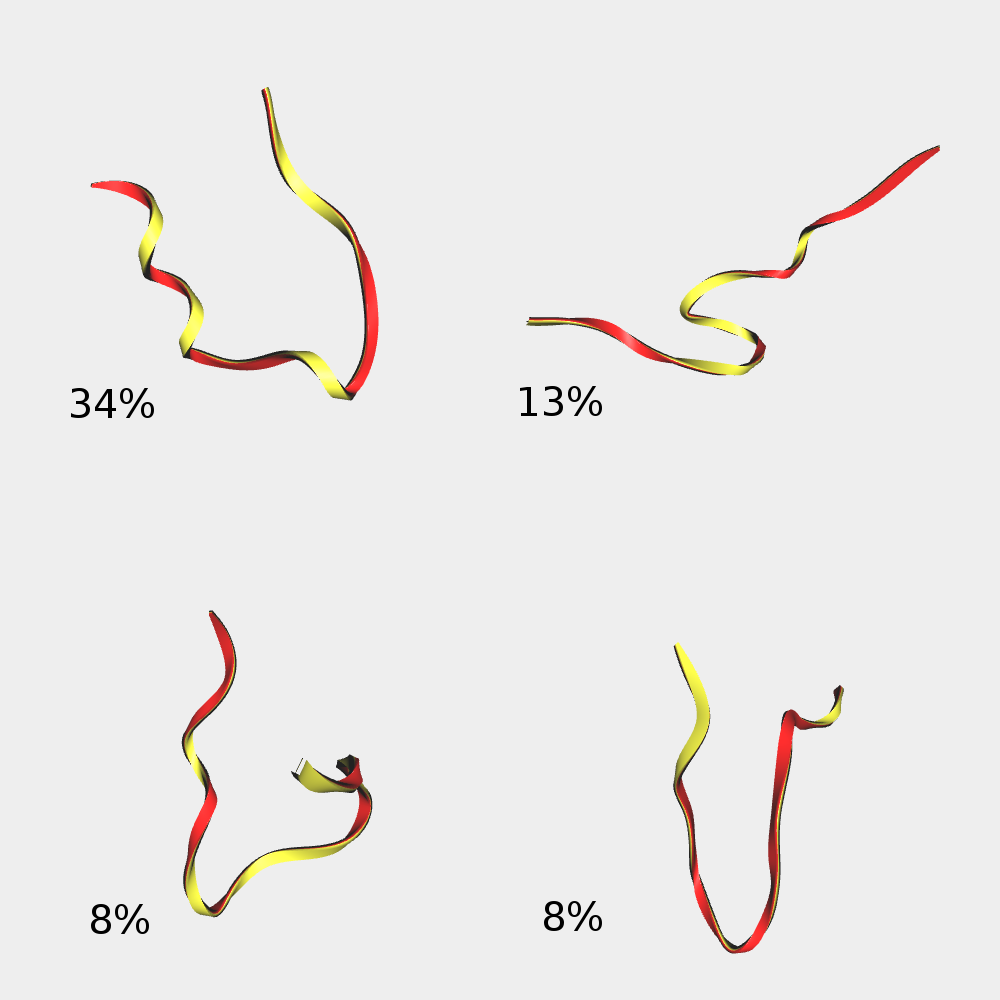
\includegraphics[width=\textwidth,height=\textheight,keepaspectratio]{pyproct_supp_clusters.png}

\protect\caption{Representative conformations for the 4 most populated clusters, holding
a 34\%, 13\%, 8 \% and 8\% of the elements of the dataset. \label{fig:clusters}}
\end{figure}

